\documentclass[11pt,a4paper]{jsarticle}

\usepackage{amsmath,amssymb}
\usepackage{bm}
\usepackage{graphicx}
\usepackage{ascmac}
\usepackage{subfigure}
\newlength{\subfigwidth}
\newlength{\subfigcolsep}

\graphicspath{{./img/}}

\title{TPC-H performance measure}
\author{Keisuke Suzuki}

\begin{document}
\maketitle
\section{実験環境}
\begin{itemize}
 \item CPU : Xeon X7560 @ 2.27GHz x4
 \item Memory : 64GB
 \item DBMS : PostgreSQL 9.2
 \item RAID0 : iodrive x8 (chunk size = 64KB)
 \item 各テーブルのprimary key上にB-tree indexを構築
 \item Scale Factor = 100
 \item shared buffer = 8GB
 \item 各クエリの実行時の状況をiostatとmpstatで1秒おきに監視
\end{itemize}

\clearpage
\section{Query 8}
簡単の為、Query8のうちのIOがメインとなる部分のみを実行する。

\subsection{Query and Execution Plan}
\begin{verbatim}
 select
	extract(year from o_orderdate) as o_year,
	l_extendedprice * (1 - l_discount) as volume,
	n2.n_name as nation
from
	part, supplier, lineitem, orders,
	customer, nation n1, nation n2,	region
where
	p_partkey = l_partkey
	and s_suppkey = l_suppkey
	and l_orderkey = o_orderkey
	and o_custkey = c_custkey
	and c_nationkey = n1.n_nationkey
	and n1.n_regionkey = r_regionkey
	and r_name = 'AMERICA'
	and s_nationkey = n2.n_nationkey
	and o_orderdate between date '1995-01-01' and date '1996-12-31'
	and p_type = 'ECONOMY ANODIZED STEEL'
\end{verbatim}

\begin{figure}[thbp]
 \begin{center}
  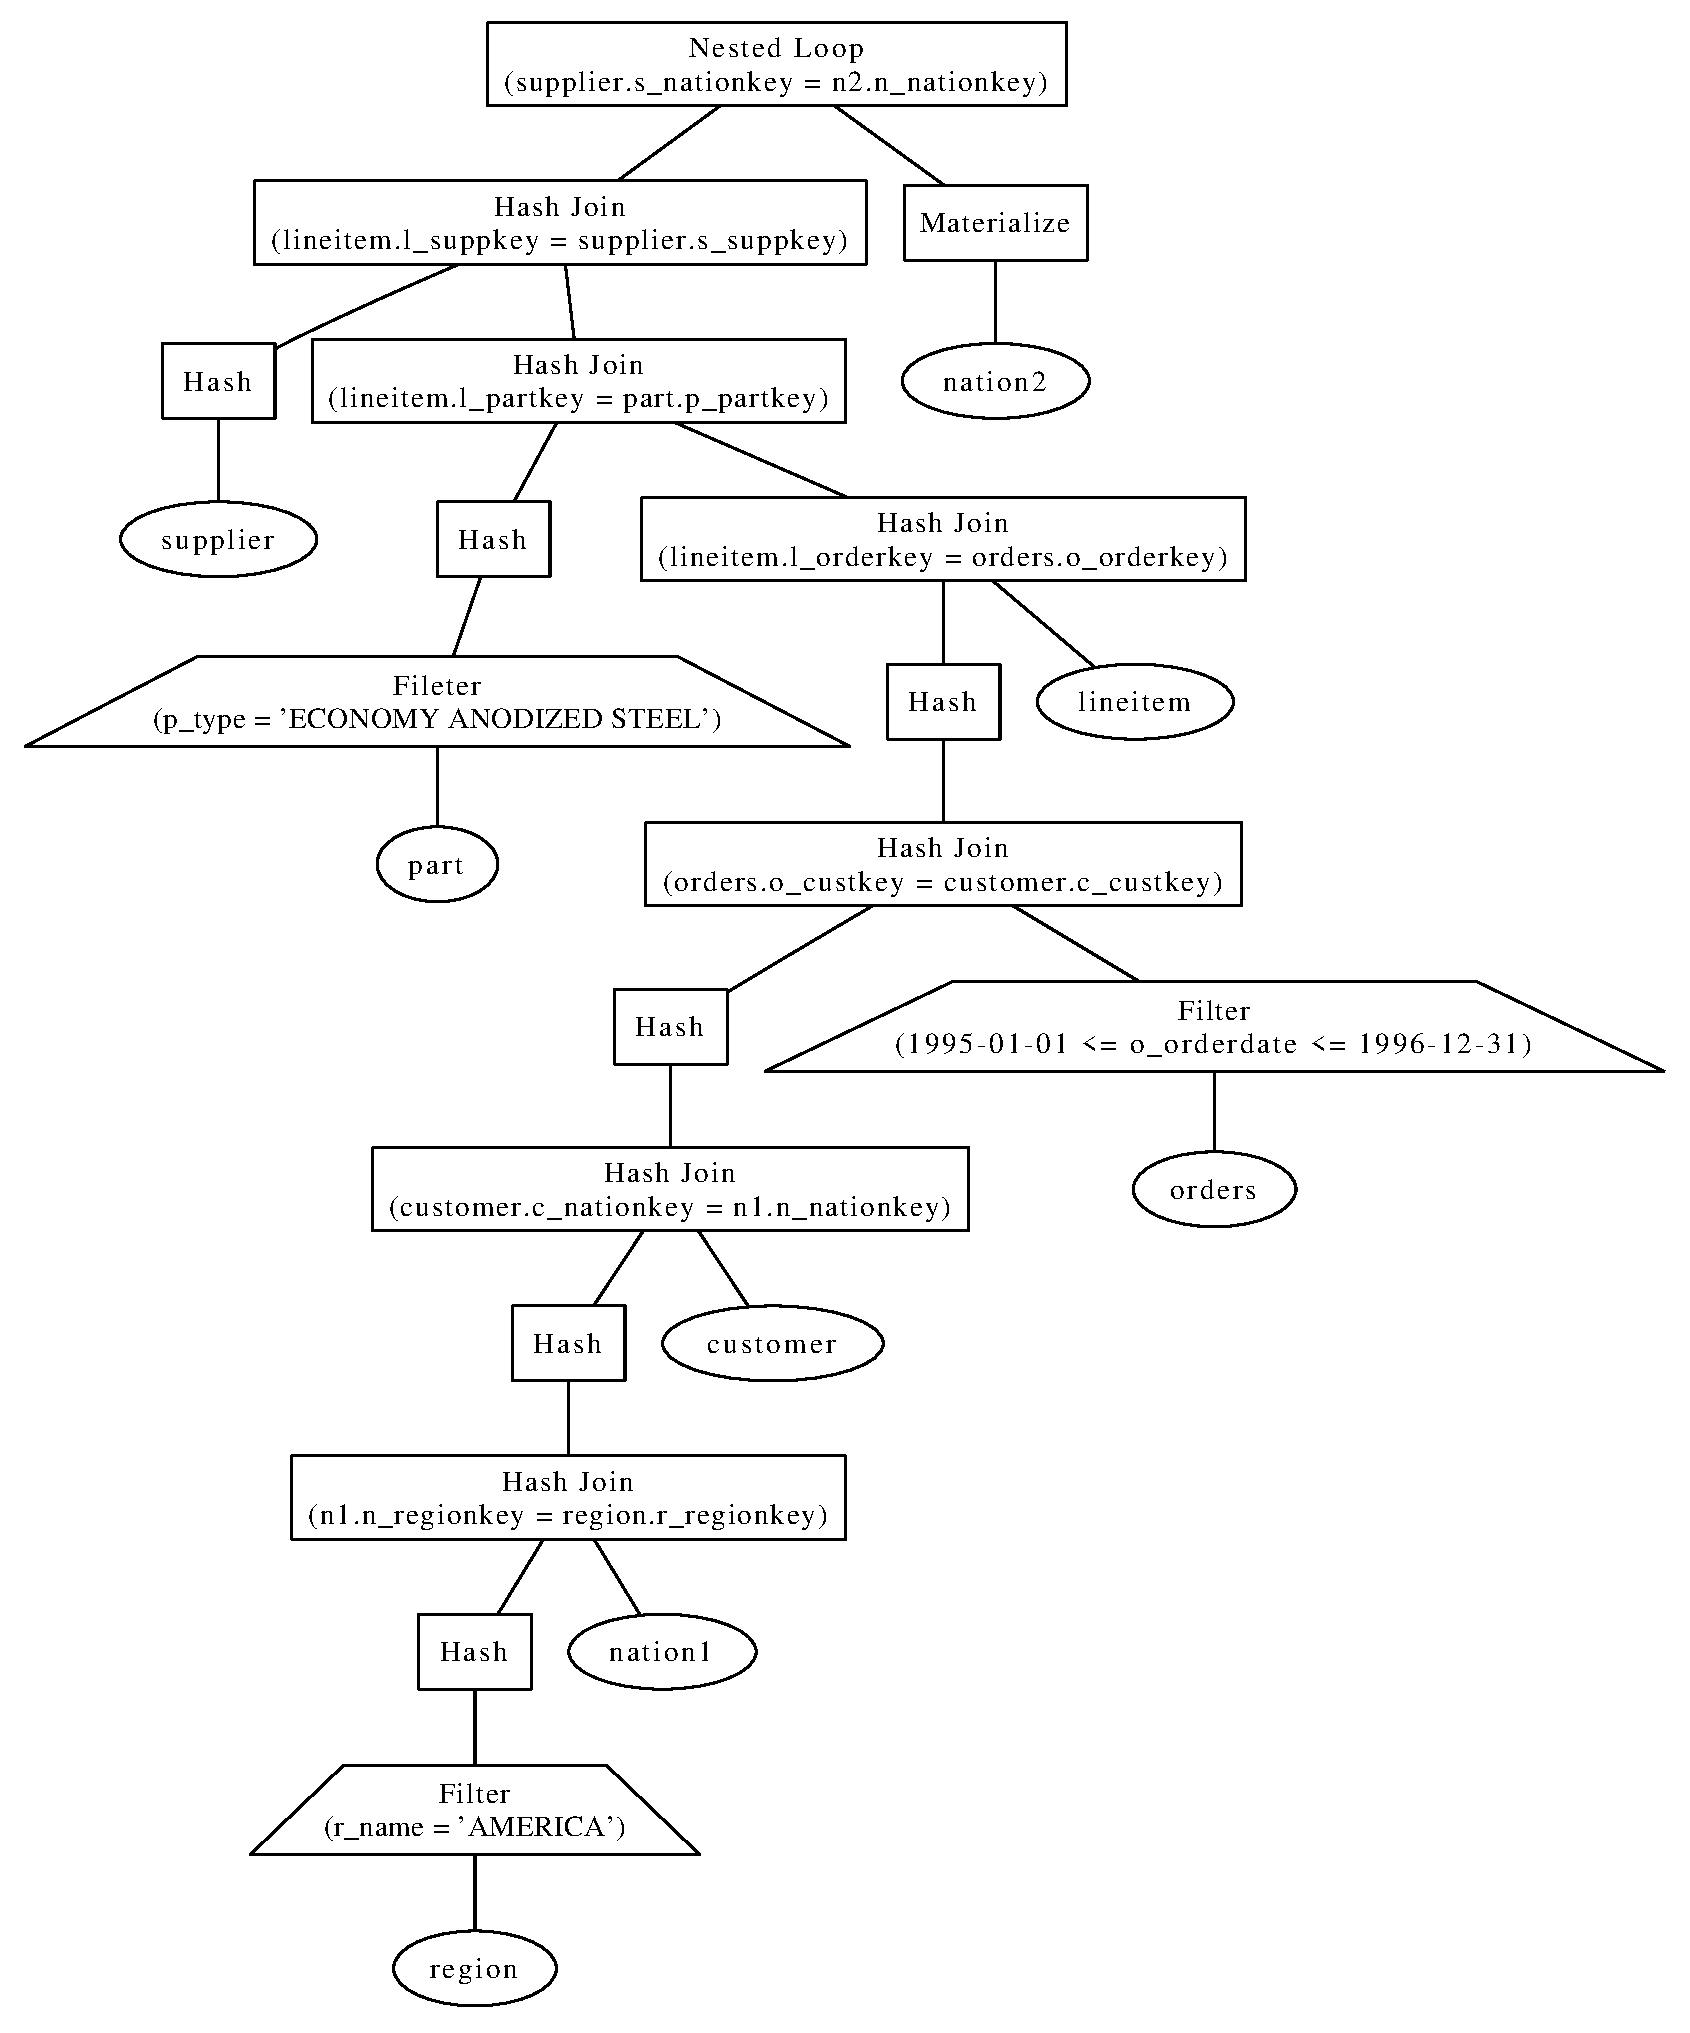
\includegraphics[width=170mm]{query8.eps}
 \end{center}
 \caption{Query 8 execution plan}
 \label{fig:query8}
\end{figure}

\clearpage
\subsection{結果}
\begin{figure}[thbp]
 \setlength{\subfigwidth}{.5\linewidth}
 \addtolength{\subfigwidth}{-.5\subfigcolsep}
 \begin{minipage}[b]{\subfigwidth}
  \subfigure[IOPS]{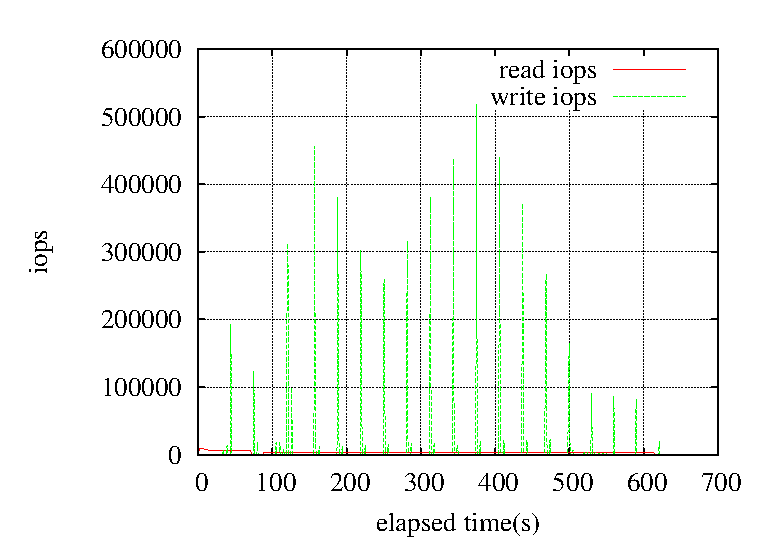
\includegraphics[width=75mm]{8coreiops.eps}
  \label{fig:8coreiops}}
 \end{minipage}
  \begin{minipage}[b]{\subfigwidth}
    \subfigure[MBPS]{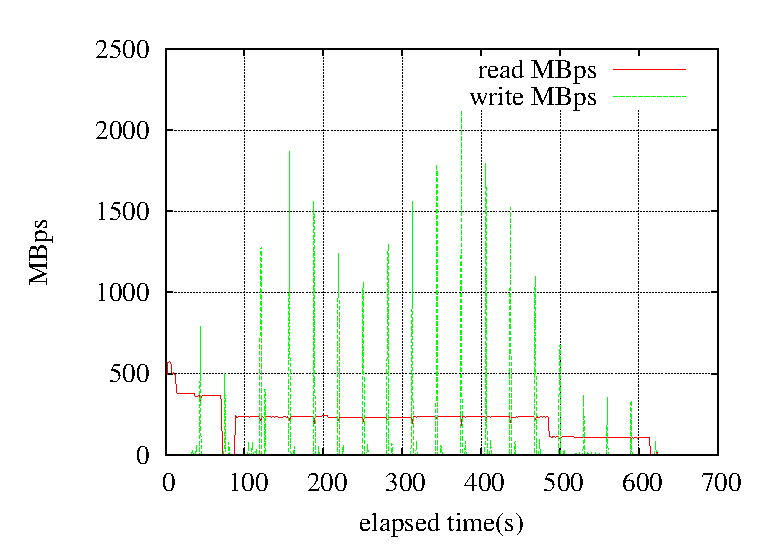
\includegraphics[width=75mm]{8corembps.eps}
   \label{fig:8corembps}}
  \end{minipage}
  \caption{IO spec}
  \label{fig:8core}
\end{figure}

\begin{figure}[thbp]
 \begin{center}
  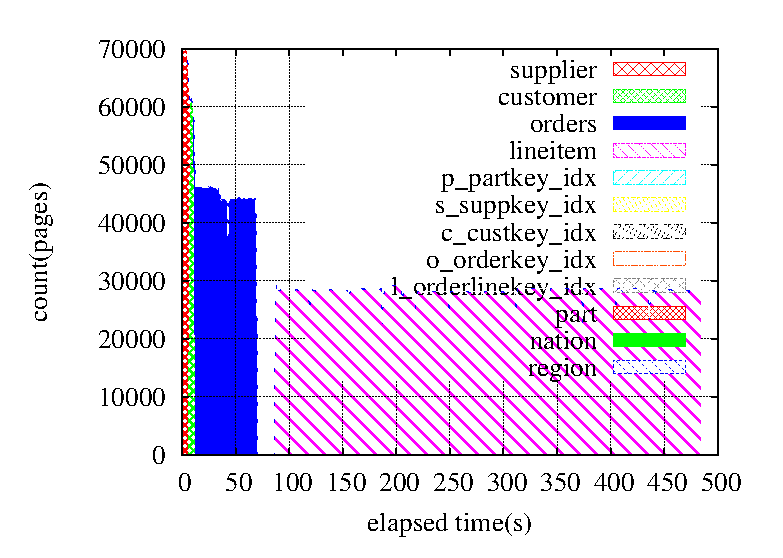
\includegraphics[width=110mm]{trace_54233refhist.eps}
 \end{center}
 \caption{detail of IO}
 \label{fig:8ioref}
\end{figure}

\end{document}
